\documentclass[11pt, A4paper,norsk]{article}
\usepackage[utf8]{inputenc}
\usepackage[T1]{fontenc}
\usepackage{babel}
\usepackage{amsmath}
\usepackage{amsfonts}
\usepackage{amsthm}
\usepackage[colorlinks]{hyperref}
\usepackage{listings}
\usepackage{color}
\usepackage{hyperref}
\usepackage{graphicx}
\usepackage{cite}
\usepackage{float}

\definecolor{dkgreen}{rgb}{0,0.6,0}
\definecolor{gray}{rgb}{0.5,0.5,0.5}
\definecolor{daynineyellow}{rgb}{1.0,0.655,0.102}
\definecolor{url}{rgb}{0.1,0.1,0.4}

\lstset{frame=tb,
	language=Python,
	aboveskip=3mm,
	belowskip=3mm,
	showstringspaces=false,
	columns=flexible,
	basicstyle={\small\ttfamily},
	numbers=none,
	numberstyle=\tiny\color{gray},
	keywordstyle=\color{blue},
	commentstyle=\color{daynineyellow},
	stringstyle=\color{dkgreen},
	breaklines=true,
	breakatwhitespace=true,
	tabsize=3
}

\lstset{inputpath="C:/Users/Torstein/Documents/UiO/Fys-Mek1110/Python programmer/Oblig1"}
\graphicspath{{C:/Users/Torstein/Documents/UiO/Fys-Mek1110/"Python programmer"/Oblig1/}}
\hypersetup{colorlinks, urlcolor=url}

\author{Torstein Solheim Ølberg}
\title{Svar på Oblig nr.1 i Fys-Mek1110}

\begin{document}
\maketitle
	\begin{center}
\Large \textbf{Oppgaver}
	\end{center}
		\paragraph{a)}
			\begin{flushleft}
A sprinter is accelerating along the track. Draw a free-body diagram of the sprinter, including only horizontal forces. Try to make the length of the vectors correspond to the relative magnitudes of the forces.
			\end{flushleft}
			\begin{flushleft}
\textbf{Løsning:}
			\end{flushleft}
			\begin{figure}
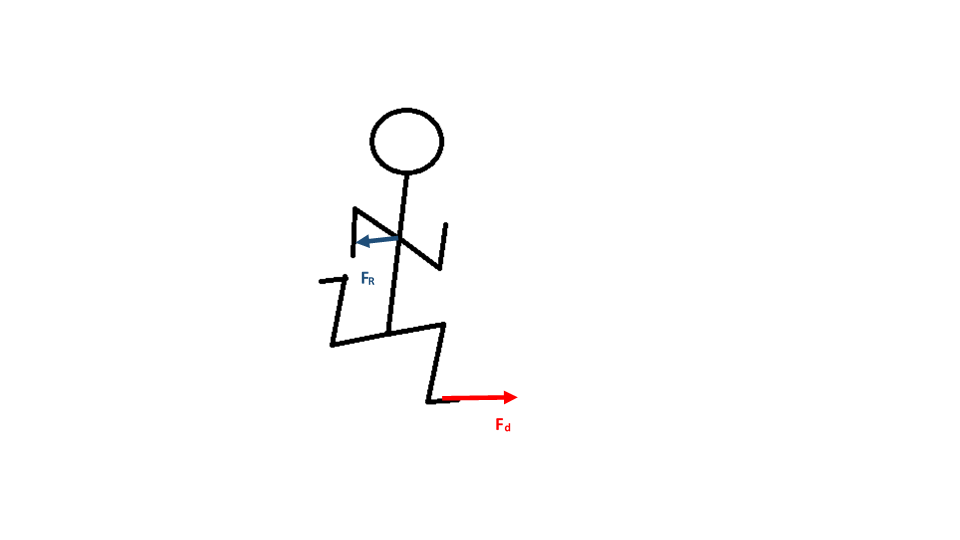
\includegraphics[width=12.6cm,height=8cm]{C:/Users/Torstein/Documents/UiO/Fys-Mek1110/Oblig1_a.png}
			\end{figure}
		\paragraph{b)}
			\begin{flushleft}
Let us assume that the sprinter is accelerated by a constant horizontal driving force, $F = 400N$, from the ground all the way from the start to the 100m line (averaged over a few steps). The mass of the sprinter is $m = 80kg$. \\
\vspace{2mm} Find the position, $x(t)$, of the sprinter as a function of time.
			\end{flushleft}
			\begin{flushleft}
\textbf{Løsning:}
			\end{flushleft}
			\begin{flushleft}
				\begin{align}
x(t) = x0 + v0t + 0.5at^{2} \\
a = \frac{F}{m} \\
x(t) = x0 + v0t + 0.5\frac{F}{m}t^{2} \\
x0 = 0, v0 = 0 \Rightarrow x(t) = 0.5\frac{F}{m}t^{2} \\
F = 400N, m = 80kg \Rightarrow x(t) = \frac{5}{2}t^{2}
				\end{align}

			\end{flushleft}
		\paragraph{c)}
			\begin{flushleft}
Show that the sprinter uses $t = 6.3s$ to reach the $100m$ line.
			\end{flushleft}
			\begin{flushleft}
\textbf{Løsning:}
			\end{flushleft}
			\begin{flushleft}
				\begin{align}
100 = \frac{5}{2}t^{2} \Rightarrow t^{2} = 40 \Rightarrow t \approx 6.3
				\end{align}
			\end{flushleft}
		\paragraph{d)}
			\begin{flushleft}
This is a bit fast compared with real races. However, real sprinters are limited by  air recistance. Let us introduce a model for air resistance by assuming that air resistance force is described by a square law:
				\begin{align}
					D = (1/2) \rho C_{D }A (v - w)^{2}
				\end{align}
where $\rho$ is the density of air, $A$ is the cross-sectional area of the runner, $C_{D}$ is the drag coefficient, $v$ is the veolcity of the runner, and $w$ is the velocity of the air. At sea level $\rho = 1.293kg/m^{3}$, and for the runner we assume $A = 0.45m^{2}$, and $C_{D} = 1.2$. You can initially assume that there is no wind: $w = 0m/s$. \\
Assume that the runner is only affected by the constant driving force, $F$, and the air resistance force, $D$. \\
\vspace{2mm} Find an expression for the acceleration of the runner.
			\end{flushleft}
			\begin{flushleft}
\textbf{Løsning:}
			\end{flushleft}
			\begin{flushleft}
				\begin{align}
\Sigma F = D + F = ma \\
a = \frac{-D + F}{m} = \frac{-0.5\rho C_{D}A(v - w)^{2} + F}{m} \label{d} \\
  = \frac{-(0.5 \cdot 1.293kg/m^{3} \cdot 1.2 \cdot 0.45m^{2} \cdot v^{2}) + 400N}{80kg} \\
= -(0.0043639v^{2} + 5)m/s^{2}
				\end{align}
Det er jo da \ref{d} likningen som er best å bruke når man eventuelt skal programmere.
			\end{flushleft}
		\paragraph{e)}
			\begin{flushleft}
Use Euler's method to find the velocity, $v(t)$, and position, $x(t)$ as a function of time for the runner. The runner starts from rest at the time $t = 0s$. Plot the positin, velocity and acceleration of the runner as a function of time. How did you decide on the time-step $\delta t$? (Your answer should include the program used to solve the problem and the resulting plots).
			\end{flushleft}
			\begin{flushleft}
\textbf{Løsning:}
			\end{flushleft}
\lstinputlisting{Oblig1_e.py}
			\begin{figure}[H]
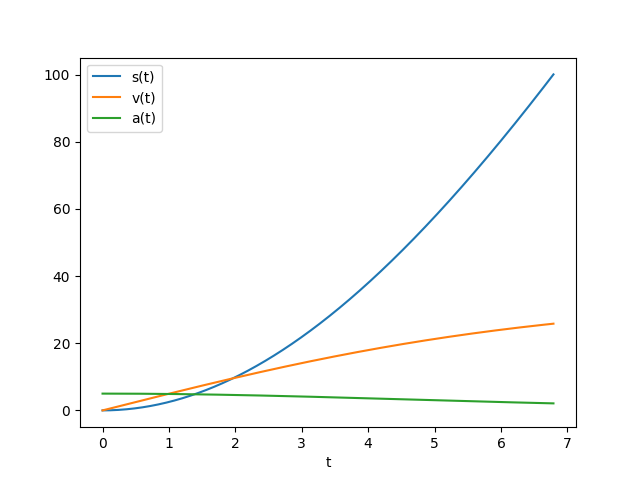
\includegraphics[width=10cm,height=8cm]{Oblig1_e.png}
			\end{figure}
Jeg valgte tidsteget 0.01 fordi dette gav et resultat på tre desimaler samtidig som at det ikke gjorde at programmet var spesielt treigt.
		\paragraph{f)}
			\begin{flushleft}
Use the result to find the race time for 100m race.
			\end{flushleft}
			\begin{flushleft}
\textbf{Løsning:}
			\end{flushleft}
				\begin{flushleft}
\lstinputlisting{Oblig1_f.py}
				\end{flushleft}
		\paragraph{g)}
			\begin{flushleft}
Show that the (theoretical) maximum velocity of a runner driven by these forces is:
				\begin{align}
v_{T} = \sqrt{\frac{2F}{\rho C_{D} A}}.
				\end{align}
The runner may have to run more than $100m$ to reach this velocity. (We often call this maximum velocity the terminal velocity - "terminal" because the velocity increases until it reaches the terminal velocity, where the acceleration becomes zero). Find the numerical value of the terminal velocity for the runner. Do you think this is realistic?
			\end{flushleft}
			\begin{flushleft}
\textbf{Løsning:}
			\end{flushleft}
				\begin{flushleft}
\lstinputlisting{Oblig1_g.py}
Som vi ser av programmet over får vi at toppfarten blir $34m/s$. Dette virker ikke som en spesielt realistisk toppfart, fordi det er rundt 3 ganger så mye som toppfarten til Usain bolt, noe som er $12,4m/s$.
				\end{flushleft}
		\paragraph{h)}
			\begin{flushleft}
If you assume that the runner is subject only to these two driving forces, what is his maximum velocity? (You can ignore the drag term, $D$, in this calculation).
			\end{flushleft}
			\begin{flushleft}
\textbf{Løsning:}
			\end{flushleft}
			\begin{flushleft}
\lstinputlisting{Oblig1_h.py}
Som vi kan se fra den numeriske analysen av formelen $a = F - F_{V}*v^{2}$ så er topphastigheten nå på $16m/s$.
			\end{flushleft}
		\paragraph{i)}
			\begin{flushleft}
Modify your numerical method to include these new forces. Find and plot x(t), v(t), a(t) for the motion.
			\end{flushleft}
			\begin{flushleft}
\textbf{Løsning:}
			\end{flushleft}
				\begin{flushleft}
\lstinputlisting{Oblig1_i.py}
				\begin{figure}[H]
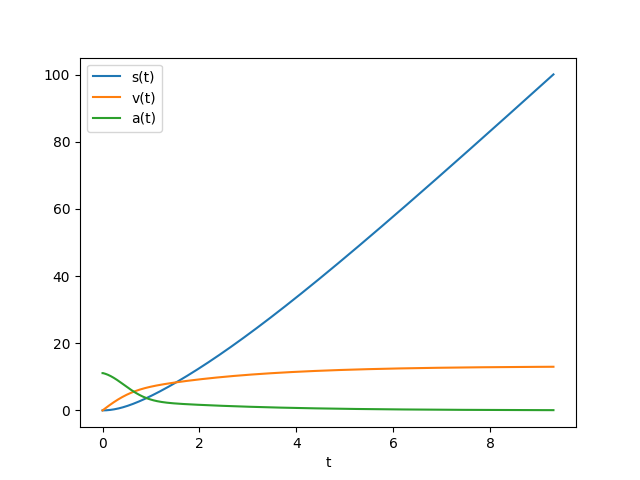
\includegraphics[width=12.6cm,height=8cm]{Oblig1_i.png}
				\end{figure}
Vi ser plottet av akselerasjonen, farten og strekningen tilbakelagt hos løperen, når vi bruker modelen vår som tar hensyn til maksfarten til en løper, luftmotstand og akselrasjonsperioden i starten av løpet.
				\end{flushleft}
		\paragraph{j)}
			\begin{flushleft}
How fast does he run $100m$?
			\end{flushleft}
			\begin{flushleft}
\textbf{Løsning:}
			\end{flushleft}
				\begin{flushleft}
\lstinputlisting{Oblig1_j.py}
Av programmet får vi at løperen bruker 9.3 sek på hele løpet. Dette er mye bedre antagelse en i oppgave g.
				\end{flushleft}
		\paragraph{k)}
			\begin{flushleft}
Compare the magnitudes of the various forces acting on the runner by plotting $F$ (which is constant), $F_{C}$, $F_{D}$ and $D$ as a function of time for a $100m$ race. Discuss how important the various effects are.
			\end{flushleft}
			\begin{flushleft}
\textbf{Løsning:}
			\end{flushleft}
				\begin{flushleft}
\lstinputlisting{Oblig1_k.py}
Kraften F(t) har en stor betydning hele tiden. Det er jo ganske selvfølgelig siden den er løperen sin kraft. FC(t), altså startakselrasjonen, har veldig stor betydning i begynnelsen, men faller fort i styrke og vil etter bare rundt 2 sekunder har den ca null betydning.
FV(t) spiller derimot ikke så veldig stor rolle det første halve sekundet ca,
men øker ganske for i betydning.
Til slutt har vi D(t) som har relativt gjevn, men liten betydning
Av dette er nok det eneste jeg ville tatt bort, hvis jeg skulle forenklet programmet, FC(t) etter 2 sek.
				\end{flushleft}
		\paragraph{l)}
			\begin{flushleft}
Use the model to test how the resulting time on 100m would change if the runner had a hind wind with a wind speed of $w = 1m/s$. What if he was running into a wind with wind speed of $w = 1m/s$?
			\end{flushleft}
			\begin{flushleft}
\textbf{Løsning:}
			\end{flushleft}
				\begin{flushleft}
\lstinputlisting{Oblig1_l.py}
Vi ser av programmet at med en medvind på 1m/s så vil han løpe på $9.21sek$, mens hvis han hadde hatt en motvind på 1m/s bruker løperen $9.43sek$
				\end{flushleft}
\end{document}